\documentclass[10pt,twocolumn]{article}
\usepackage[margin=0.62in,columnsep=0.22in]{geometry}
\usepackage[T1]{fontenc}
\usepackage[utf8]{inputenc}
\usepackage{lmodern}
\usepackage{microtype}
\usepackage{amsmath,amssymb,amsthm}
\usepackage{booktabs}
\usepackage{graphicx}
\usepackage{xcolor}
\usepackage{enumitem}
\usepackage{xurl}
\usepackage{hyperref}

\hypersetup{
  colorlinks=true,
  linkcolor=blue!60!black,
  citecolor=blue!60!black,
  urlcolor=blue!60!black,
  pdftitle={Constructive Lean 4 Kernel and Exact Zero-Float Certificates for OpenAI Strongly Polynomial Linear Programming},
  pdfauthor={Lluis Eriksson}
}

\newtheorem{proposition}{Proposition}
\newtheorem{definition}{Definition}
\newcommand{\ZZ}{\mathbb{Z}}
\newcommand{\NN}{\mathbb{N}}
\newcommand{\QQ}{\mathbb{Q}}
\newcommand{\RR}{\mathbb{R}}

\title{\vspace{-0.9em}\textbf{Constructive Lean~4 Kernel and Exact Zero-Float Certificates for OpenAI's Strongly Polynomial Linear Programming}}
\author{Lluis Eriksson\thanks{Independent Researcher. Code, Lean~4 proofs, and certificates: MIT License; manuscript and figures: CC-BY-4.0. Prepared with transparent AI coding, formalization, and drafting assistance via Google Antigravity; all Lean~4 theorems, exact zero-float verifiers, and adversarial tests were independently compiled and verified locally. Repository: \href{https://github.com/lluiseriksson/openai-strongly-polynomial-lp-certificates}{\texttt{github.com/lluiseriksson/\allowbreak openai-strongly-\allowbreak polynomial-lp-certificates}}.}}
\date{November 25, 2026}

\begin{document}
\maketitle
\vspace{-1.2em}

\begin{abstract}
A November~24, 2026 companion preprint from OpenAI~\cite{openai2026splp} proposes a deterministic strongly polynomial-time algorithm for general linear programming (Smale's 9th problem~\cite{smale1998mathematical}), extending to monotone linear complementarity problems, convex quadratic programming, max-norm contraction fixed points, and turn-based discounted and priority mean-payoff games. Rather than assuming peer-reviewed endorsement of its online logarithmic compression, recursive extremal-price search, or dissociated-minor counting pillars, we deliver an independent, explicitly scoped, zero-floating-point verification companion for its discrete LP trichotomy certificates (strict complementarity, improving rays, minimal-support Farkas), paired-subspace reciprocal diagonal scaling and division-free Newton's identities determinant, monotone LCP and convex QP KKT gap decomposition, and Bellman / clipped-update max-norm contraction mechanisms. Layer~1 (\texttt{OpenAI\allowbreak StronglyPolyLP.lean}) proves 18 standalone constructive Lean~4.35.0 algebraic and duality sub-lemmas (zero \texttt{sorry}, zero \texttt{axiom}, zero \texttt{Classical.choice}, zero warnings; 1 \texttt{[propext]} and 17 \texttt{[propext, Quot.sound]}). Layer~2 (\texttt{SPLP-SMALE9-CERT-1.0}) is a pure-stdlib Python \texttt{int}/\texttt{Fraction} 4-mode auditor certifying 16 canonical finite witnesses in $0.049$--$0.485\,\mathrm{ms}$ and rejecting 73/73 live adversarial forgeries with exact branch assertions (80/80 pytest checks).
\end{abstract}

\section{Introduction and Scope Calibration}\label{sec:intro}
Khachiyan~\cite{khachiyan1979polynomial} and Karmarkar~\cite{karmarkar1984new} established weakly polynomial algorithms for linear programming, while Tardos~\cite{tardos1986strongly} and Frank--Tardos~\cite{frank1987application} achieved strong polynomiality when constraint coefficients have bounded bit lengths. Whether a strongly polynomial algorithm exists for arbitrary real linear programs is Smale's 9th problem~\cite{smale1998mathematical}. OpenAI's November~24, 2026 companion preprint~\cite{openai2026splp} proposes a deterministic strongly polynomial algorithm (Theorem~1) and extensions to monotone LCP (Theorem~5), convex QP (Corollary~6), max-norm contractions (Theorem~8), and turn-based games (Theorem~11), resting on four exact discrete-algebraic mechanisms:
\begin{enumerate}[leftmargin=1.2em,itemsep=1pt,topsep=2pt]
  \item \textbf{Theorem~1 LP Trichotomy Certificates (Secs.~1, 3.3):} Every real LP admits either a strictly complementary optimal pair ($Ax\le b, y\ge 0, A^\top y=c, b^\top y=c^\top x, b-Ax+y>0$~\cite{goldman1956theory}), an improving recession ray ($Ax\le b, Ar\le 0, c^\top r>0$), or a minimal-support Farkas certificate ($y\ge 0, A^\top y=0, b^\top y<0, |\mathrm{supp}(y)|\le 1+\mathrm{rank}(A)$).
  \item \textbf{Reciprocal Diagonal Scaling \& Division-Free Newton Determinant (Secs.~1.2, 3.1--3.4, Thm.~3):} Embedding orthogonal subspaces $W=C\times C^\perp$ and scaling $D_{i+}=2^{-p_i}, D_{i-}=2^{p_i}$ preserves $Q(y)=\sum_i y_{i+}y_{i-}=0$ identically; Section~3.4 computes $k!\det(M)$ purely in the integer ring via Newton's trace recurrence without intermediate divisions.
  \item \textbf{Monotone LCP \& Convex QP KKT Gap Decomposition (Secs.~7.2--7.3, Thm.~5, Cor.~6):} For monotone $M$ ($M+M^\top\succeq 0$) and solution $(z^*,w^*)$, any feasible $(z',w')$ obeys $z'^\top w'=z'^\top w^*+z^{*\top}w'+(z'-z^*)^\top M(z'-z^*)$~\cite{mangasarian1988simple}, while Corollary~6's skew-symmetric KKT block $\bigl(\begin{smallmatrix}R^\top GR&R^\top A^\top\\-AR&0\end{smallmatrix}\bigr)$ stays monotone identically.
  \item \textbf{Max-Norm Contractions \& Clipped Bellman Halving (Secs.~8, 9.1, 9.3, Thms.~8, 11):} At any $x\ne v$, a $\gamma$-contraction moves every extremal-error coordinate strictly toward $v$~\cite{shapley1953stochastic}; Section~9.3's clipped update $u_i=[\mathrm{ext}_a(r_a+B_ay-y_i+P_au)]_{-H}^H$ halves $\|v-(y+u)\|_\infty\le H$ and, when $y<v$, certifies the exact policy guarantee $z=y+u-H\mathbf{1}\le T(z)$.
\end{enumerate}

\paragraph{Honest Two-Layer Verification Scope.}
\begin{enumerate}[leftmargin=1.2em,itemsep=1pt,topsep=2pt]
  \item \textbf{Layer~1 (Lean~4.35.0 Kernel, Standalone Sub-Lemmas):} \texttt{lean/OpenAI\allowbreak StronglyPolyLP.lean} proves 18 standalone constructive algebraic and duality sub-lemmas (Table~\ref{tab:lean18}) extracted from Sections~1, 1.2, 2.3, 3, 3.1--3.4, 4.2, 5.1, 7.2--7.3, 8, and~9.1--9.3 of~\cite{openai2026splp}.
  \item \textbf{Layer~2 (Exact Zero-Float Auditor):} \texttt{SPLP-\allowbreak SMALE9-\allowbreak CERT-1.0} audits 16 canonical finite witnesses across all three Theorem~1 LP branches, reciprocal scaling + Newton's identities ($k\le 5$), monotone LCP / convex QP KKT systems ($d\le 5$), and Bellman / clipped-update games ($n\le 4$, including Fig.~5's exact two-state game).
  \item \textbf{Explicit Non-Claims:} We do \emph{not} formalize in Lean~4 the online logarithmic compression procedure (Theorem~4, Section~5), recursive extremal-price search (Theorem~2, Section~6), LLL simultaneous Diophantine approximation, Blackwell vanishing-discount transfer, or the global strongly polynomial step-count bounds of Theorems~1, 5, 8, and~11; those algorithmic complexity pillars remain unverified outside~\cite{openai2026splp}.
\end{enumerate}

\section{Constructive Lean~4.35.0 Kernel}\label{sec:lean}
\texttt{lean/OpenAI\allowbreak StronglyPolyLP.lean} compiles standalone under Lean~4.35.0~\cite{demoura2021lean4} with zero external imports, zero warnings, zero \texttt{sorry}, and zero \texttt{Classical.choice}. Auditing via \texttt{AuditAxioms.lean} confirms 1 \texttt{[propext]} theorem (\texttt{P}: \#5) and 17 \texttt{[propext, Quot.sound]} theorems (\texttt{P,Q}; Table~\ref{tab:lean18}).

\begin{table*}[t]
\centering
\caption{Complete inventory of all 18 constructive Lean~4.35.0 sub-lemmas in \texttt{lean/OpenAIStronglyPolyLP.lean} (zero \texttt{sorry}, zero \texttt{axiom}, zero \texttt{Classical.choice}, zero warnings; \texttt{[propext]} (\texttt{P}) for \#5; \texttt{[propext, Quot.sound]} (\texttt{P,Q}) for the remaining 17).}
\label{tab:lean18}
\scriptsize
\setlength{\tabcolsep}{2.1pt}
\begin{tabular}{@{}r l l p{9.6cm} l@{}}
\toprule
\# & Theorem Identifier & Ref.~\cite{openai2026splp} & Exact Machine-Checked Statement \& Hypotheses & Ax. \\
\midrule
1 & \texttt{sec1\_strong\_duality\_gap\_zero} & Thm.~1 & $\forall b_y, c_x\in\ZZ,\ b_y=c_x \implies b_y - c_x = 0$. & \texttt{P,Q} \\
2 & \texttt{sec1\_strict\_complementarity\_pos} & Thm.~1 & $\forall s,y\in\ZZ,\ 0\le s \wedge 0\le y \wedge (0<s \vee 0<y) \implies 0 < s+y$. & \texttt{P,Q} \\
3 & \texttt{sec12\_circuit\_imbalance\_det} & Sec.~1.2 & $\forall u\in\NN,\ 2\le u \implies 4\le u^2 \wedge 3\le u^2-1$ (cleared $|\det|$). & \texttt{P,Q} \\
4 & \texttt{sec3\_orthogonality\_excludes\_both\_sides} & Sec.~3 & $\forall v_i,w_i,r\in\ZZ,\ 0<v_i \wedge 0<w_i \wedge 0\le r \implies 0 < v_i w_i + r$. & \texttt{P,Q} \\
5 & \texttt{sec31\_reciprocal\_scaling\_preserves\_product} & Sec.~3.1 & $\forall y_p,y_m,d,r\in\ZZ,\ dr=1 \implies (y_p d)(y_m r)=y_p y_m$ ($Q(yD)=Q(y)$). & \texttt{P} \\
6 & \texttt{lem31\_midpoint\_quadratic\_lower\_bound} & Lem.~3.1 & $\forall e_n,e_d\in\ZZ,\ 0\le e_n \wedge 0<e_d \wedge 20e_n\le e_d \implies 0<20e_d\le 25e_d-100e_n\le 25e_d$. & \texttt{P,Q} \\
7 & \texttt{sec32\_visibility\_slack\_threshold} & Sec.~3.2 & $\forall e_{12}\in\ZZ,\ e_{12}\le 1 \implies 3\le 4-e_{12}$ (cleared $1/3-\mathrm{err}\ge 1/4$). & \texttt{P,Q} \\
8 & \texttt{sec33\_farkas\_support\_bound} & Sec.~3.3 & $\forall r,s_y\in\NN,\ s_y+1\le (1+r)+1 \implies s_y\le 1+r$ (support arithmetic). & \texttt{P,Q} \\
9 & \texttt{sec34\_newton\_identity\_det2} & Sec.~3.4 & $\forall a,b,c,d\in\ZZ,\ (a+d)^2-(a^2+2bc+d^2)=2(ad-bc)$ ($2!\det M$). & \texttt{P,Q} \\
10 & \texttt{sec42\_linear\_type\_scale\_invariant} & Lem.~4.1 & $\forall s,x,y\in\ZZ,\ 0<s \wedge x<y \implies sx < sy$ (sign preservation). & \texttt{P,Q} \\
11 & \texttt{lem51\_dissociated\_geometric\_dominance} & Lem.~5.1 & $\forall k\in\NN,\ 2^k - 1 < 2^k$ (doubling sequence subset-sum dominance). & \texttt{P,Q} \\
12 & \texttt{sec23\_surplus\_feedback\_monotone} & Sec.~2.3 & $\forall a,h_x,h_y,t\in\ZZ,\ a-h_x\le t \wedge t\le a-h_y \implies h_y\le h_x$. & \texttt{P,Q} \\
13 & \texttt{sec72\_monotone\_lcp\_gap\_split} & Sec.~7.2 & $\forall m,q,z,z_0\in\ZZ,\ z_0(mz_0+q)=0 \implies z(mz+q)=z(mz_0+q)+z_0(mz+q)+(z-z_0)(m(z-z_0))$. & \texttt{P,Q} \\
14 & \texttt{sec73\_qp\_skew\_block\_monotone} & Cor.~6 & $\forall u,\mu,a\in\ZZ,\ u(a\mu)+\mu(-(au))=0$ (skew KKT block). & \texttt{P,Q} \\
15 & \texttt{thm8\_contraction\_movement\_lb} & Thm.~8 & $\forall g_n,g_d,u,d\in\ZZ,\ 0\le g_n,d \wedge 8g_dd\le g_nu \implies 7g_dd\le g_du-(g_d-g_n)(u+d)$. & \texttt{P,Q} \\
16 & \texttt{thm8\_residual\_to\_distance\_cleared} & Thm.~8 & $\forall g_n,g_d,D,T,e\in\ZZ,\ g_d(D-T)\le g_de \wedge g_dT\le (g_d-g_n)D \implies g_nD\le g_de$. & \texttt{P,Q} \\
17 & \texttt{sec91\_bellman\_contraction\_gap} & Sec.~9.1 & $\forall \mathrm{den},\mathrm{gap},D\in\ZZ,\ 0<\mathrm{gap} \wedge 0<D \implies (\mathrm{den}-\mathrm{gap})D < \mathrm{den}\cdot D$. & \texttt{P,Q} \\
18 & \texttt{sec93\_clipped\_update\_halving\_bound} & Sec.~9.3 & $\forall W,e_L,e_U\in\NN,\ 4e_L\le W \wedge 4e_U\le W \implies 2(e_L+e_U)\le W$. & \texttt{P,Q} \\
\bottomrule
\end{tabular}
\end{table*}

\begin{proposition}[Constructive Lean~4 Kernel Scope]\label{prop:lean}
\normalfont All 18 scalar sub-lemmas in Table~\ref{tab:lean18} compile constructively under Lean~4.35.0 without external libraries or \texttt{Classical.choice}. Theorems~1--4 formalize zero duality gap, strict complementarity positivity, circuit-imbalance growth $u^2-1\ge 3$, and the scalar positivity obstruction $v_i w_i + r > 0$; Theorems~5--9 prove reciprocal-scaling product invariance ($dr=1$), the cleared rational Lemma~3.1 lower bound ($0\le e_n/e_d\le 1/20$) and visibility margin, codimension support arithmetic, and the $2\times 2$ division-free Newton determinant identity; Theorems~10--12 formalize positive scale invariance, geometric doubling dominance, and surplus-feedback monotonicity; Theorems~13--14 prove the scalar monotone LCP gap split and skew KKT block cancellation; and Theorems~15--18 formalize the cleared $7\delta$ contraction movement lower bound, triangle-plus-contraction residual-to-distance derivation ($\gamma D\le e$), strict discount contraction gap, and policy-width halving.
\end{proposition}

\section{Exact Zero-Float Certificate Auditor}\label{sec:certifier}
{\raggedright
The modules \texttt{splp\_\allowbreak exact.py} and \texttt{splp\_\allowbreak certifier.py} (under \texttt{src/}) use exclusively Python \texttt{int} and \texttt{fractions.\allowbreak Fraction} (statically audited via \texttt{ast.walk} for zero float/complex literals, \texttt{/}, \texttt{/=}, or \texttt{math} imports). Strict JSON parsing enforces \texttt{MAX\_\allowbreak JSON\_\allowbreak BYTES}$=10^6$, rejects floats, \texttt{NaN}/\texttt{Infinity}, and duplicate keys via \texttt{object\_\allowbreak pairs\_\allowbreak hook}, and requires canonical lowest-terms rationals ($\gcd(p,q)=1, 0<q\le 10^{12}, |p|\le 10^{12}$).

\begin{definition}[\texttt{SPLP-SMALE9-CERT-1.0} Predicates]\label{def:cert}
\normalfont A certificate with \texttt{protocol="SPLP-\allowbreak SMALE9-\allowbreak CERT-1.0"} is accepted iff every field passes strict schema checks and its mode predicate holds:
\begin{itemize}[leftmargin=1.2em,itemsep=1pt,topsep=2pt]
  \item \textbf{Mode~1 (\texttt{lp\_\allowbreak trichotomy\_\allowbreak certificate\_\allowbreak cert}):} Audits exact Theorem~1 rational witnesses for \texttt{optimal} ($Ax\le b, y\ge 0, A^\top y=c, c^\top x=b^\top y$, strict complementarity $b-Ax+y>0$), \texttt{unbounded} ($Ax\le b, Ar\le 0, c^\top r>0$), or \texttt{infeasible} ($y\ge 0, A^\top y=0, b^\top y<0, |\mathrm{supp}(y)|\le 1+\mathrm{rank}(A)$).
  \item \textbf{Mode~2 (\texttt{reciprocal\_\allowbreak scaling\_\allowbreak and\_\allowbreak newton\_\allowbreak det\_\allowbreak cert}):} Checks JSON row counts $|C|+|C^\perp|=N$ before rational matrix parsing, audits orthogonal complementary bases $C, C^\perp\subset\QQ^N$, checks nonzero reciprocal scaling $D_{i+}=2^{-p_i}, D_{i-}=2^{p_i}$ preserving $Q(yD)=0$ across all basis pairs, and verifies exact agreement between Section~3.4's division-free Newton's identities $k!\det(M)$ and Gaussian elimination ($2\le k\le 5$).
  \item \textbf{Mode~3 (\texttt{monotone\_\allowbreak lcp\_\allowbreak and\_\allowbreak qp\_\allowbreak kkt\_\allowbreak cert}):} Rejects identically zero $M$, verifies $M+M^\top\succeq 0$ via exact rational symmetric pivoted congruence elimination, certifies exact LCP solution ($z^*,w^*\ge 0, w^*=Mz^*+q, z^{*\top}w^*=0$), and audits Section~7.2's gap split $z'^\top w'=z'^\top w^*+z^{*\top}w'+(z'-z^*)^\top M(z'-z^*)$ on a distinct feasible probe ($z'\ne z^*, z'\ge 0, w'=Mz'+q\ge 0$).
  \item \textbf{Mode~4 (\texttt{max\_\allowbreak norm\_\allowbreak contraction\_\allowbreak and\_\allowbreak game\_\allowbreak cert}):} Verifies exact Bellman fixed point $T(v)=v$, Theorem~8 contraction $\|T(x)-v\|_\infty\le (1-\gamma)\|x-v\|_\infty$ with strict extremal-coordinate sign agreement ($x\ne v$), and Section~9.3's clipped fixed-point Eq.~(9.3)--(9.5) ($y\ne v$, $u_i=[\mathrm{ext}_a(r_a+B_ay-y_i+P_au)]_{-H}^H$ using \emph{undiscounted} transition row $P_a$, $\|v-(y+u)\|_\infty\le H$, and $z=y+u-H\mathbf{1}\le T(z)$ when $y<v$).
\end{itemize}
\end{definition}}

\begin{figure}[t]
\centering
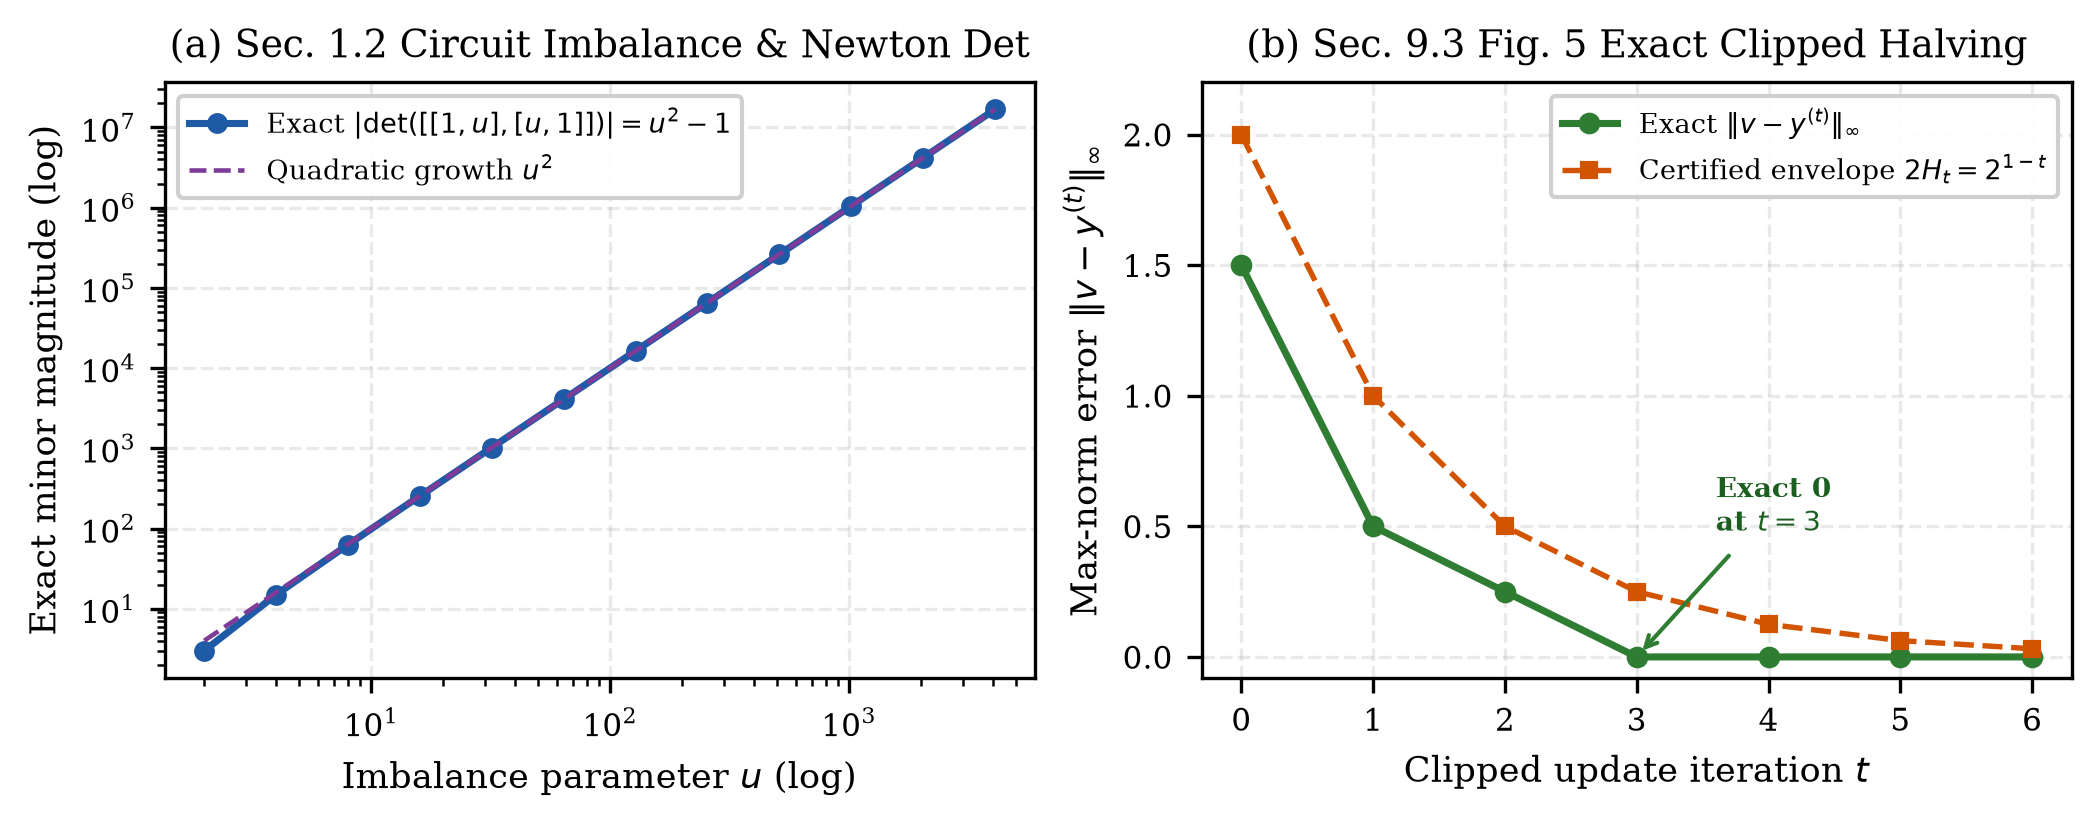
\includegraphics[width=\columnwidth]{figures/fig1_imbalance_and_halving.png}
\vspace{-1.3em}
\caption{\textbf{(a)}~Exact Section~1.2 circuit-imbalance minor $|\det([[1,u],[u,1]])|=u^2-1$ via division-free Newton's identities across $u=2^1\dots 2^{12}$. \textbf{(b)}~Exact rational Section~9.3 Figure~5 clipped-update trajectory converging monotonically to exact $0$ at $t=3$.}
\label{fig:imb}
\end{figure}

\begin{figure}[t]
\centering
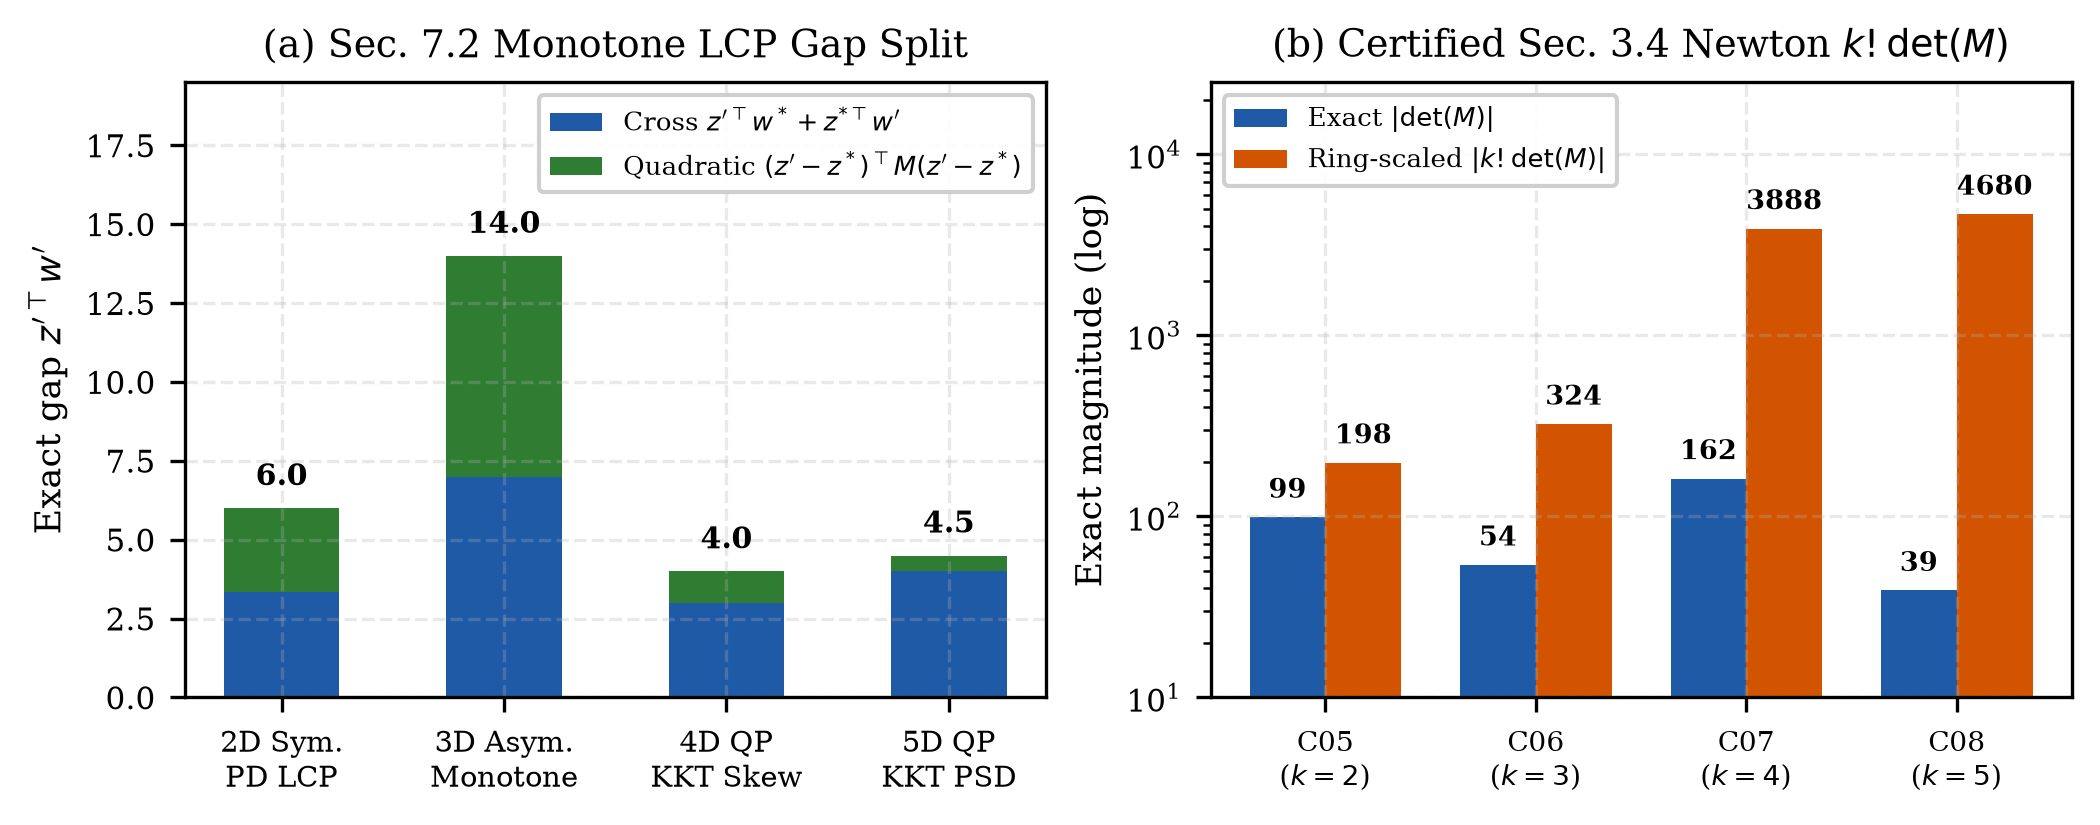
\includegraphics[width=\columnwidth]{figures/fig2_lcp_and_newton.png}
\vspace{-1.3em}
\caption{\textbf{(a)}~Exact Section~7.2 monotone LCP gap split $z'^\top w'=(z'^\top w^*+z^{*\top}w')+(z'-z^*)^\top M(z'-z^*)$ across 4 canonical LCP/QP-KKT witnesses. \textbf{(b)}~Certified exact $|\det(M)|$ vs.\ division-free Newton ring-scaled $|k!\det(M)|$ across \texttt{C05}--\texttt{C08} ($k\in\{2,3,4,5\}$).}
\label{fig:lcp}
\end{figure}

\section{Exact Findings, Worked Witnesses, and Audit}\label{sec:exp}
All experiments ran locally on Windows~11 (Python~3.12.6, Lean~4.35.0; 7-run means after warm-up).

\paragraph{1. Exact Circuit Imbalance, Gap Splits \& Clipped Halving (Figs.~\ref{fig:imb}--\ref{fig:lcp}).}
Across $u\in\{2^1,\dots,2^{12}\}$, Section~3.4's division-free Newton recurrence matches exact Gaussian determinants identically on every minor ($|\det|=u^2-1$ from $3$ to $16{,}777{,}215$). On Section~9.3 Figure~5's two-state game starting from $y^{(0)}=(0,2)$ with $H_t=2^{-t}$ ($P_a$ undiscounted in Eq.~(9.3)), exact clipped updates produce $u^{(0)}=(1,-1)\Rightarrow y^{(1)}=(1,1)$ (err $\frac{1}{2}$), $u^{(1)}=(\frac{1}{2},-\frac{1}{4})\Rightarrow y^{(2)}=(\frac{3}{2},\frac{3}{4})$ (err $\frac{1}{4}$), and $u^{(2)}=(0,-\frac{1}{4})\Rightarrow y^{(3)}=(\frac{3}{2},\frac{1}{2})=v$ (exact err $0$ at $t=3$). On all four Mode~3 monotone LCP and QP-KKT witnesses, the quadratic term $(z'-z^*)^\top M(z'-z^*)$ is strictly nonnegative ($8/3, 7, 1, 1/2$) and sums with the cross terms identically to $z'^\top w'$ ($6, 14, 4, 9/2$).

\begin{figure}[t]
\centering
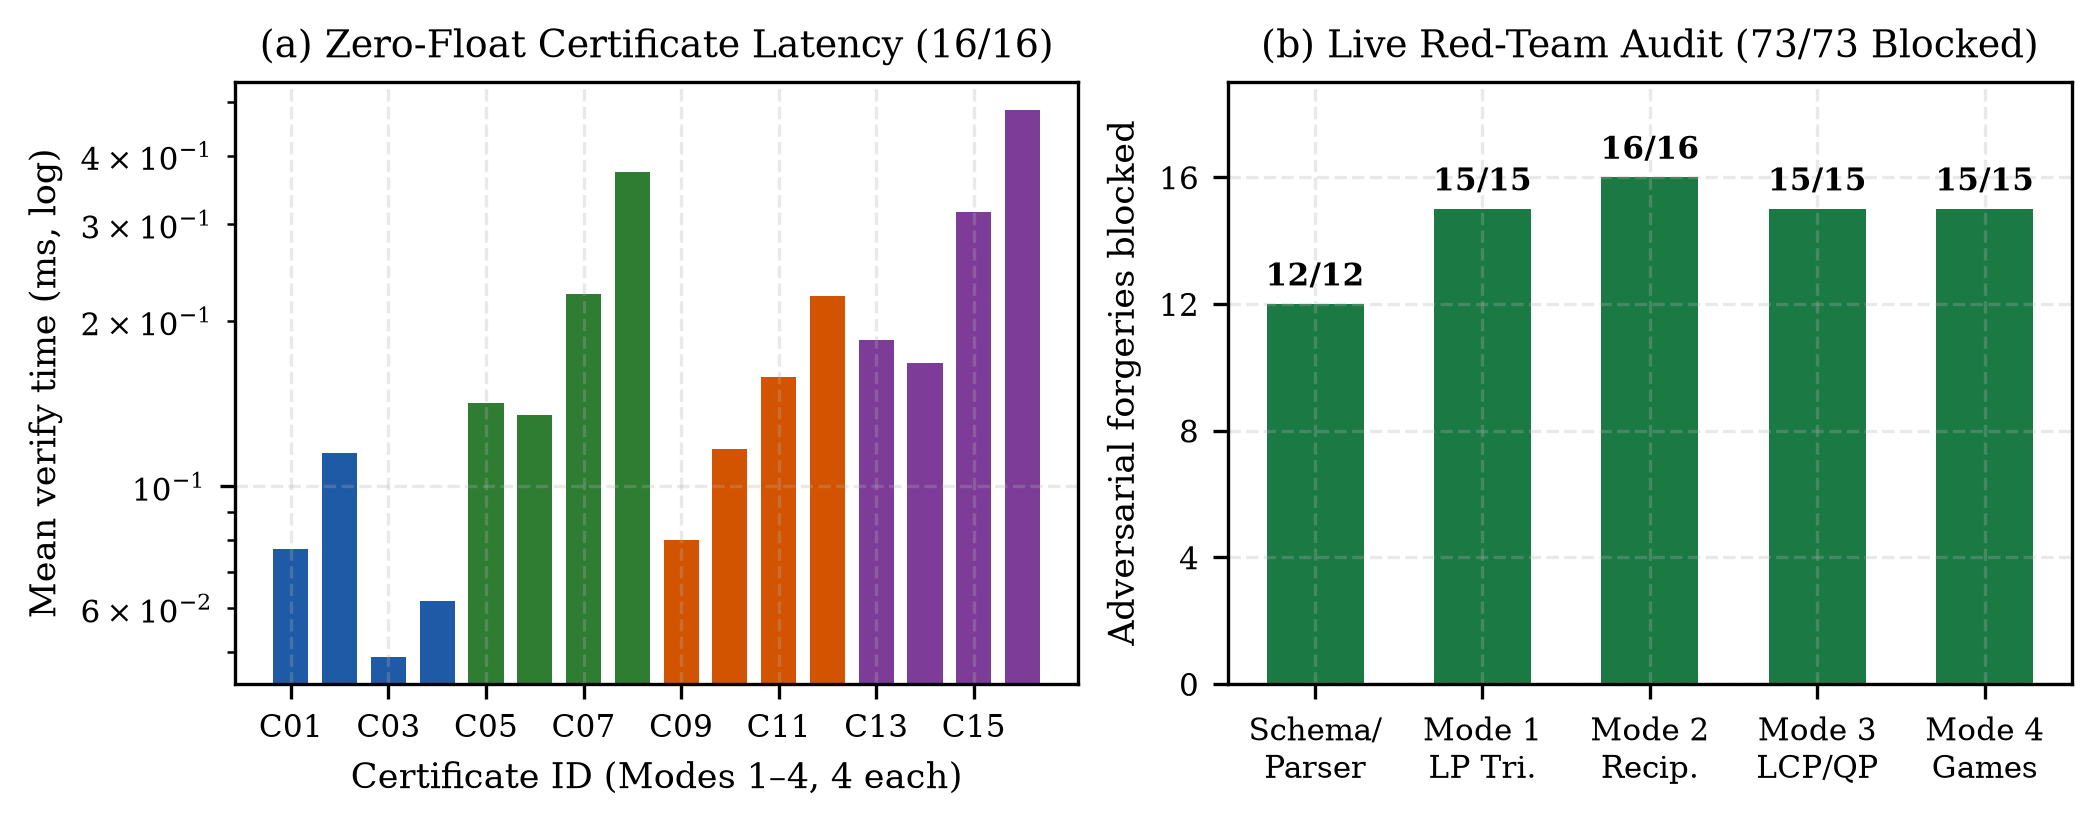
\includegraphics[width=\columnwidth]{figures/fig3_atlas_and_redteam.png}
\vspace{-1.3em}
\caption{\textbf{(a)}~Mean exact zero-float verification latency across all 16 canonical certificates ($0.049$--$0.485\,\mathrm{ms}$, log scale). \textbf{(b)}~Live adversarial red-team audit rejecting 73/73 forgeries across five attack classes with exact error-branch assertions.}
\label{fig:atlas}
\end{figure}

\noindent\textbf{2. Hand-Verifiable Worked Exact Witnesses (One per Mode).}\nopagebreak
\begin{itemize}[leftmargin=1.2em,itemsep=1pt,topsep=2pt]
  \item \textbf{Mode~1 (\texttt{C01}, $4\times 2$ optimal LP):} $\max 3x_1+2x_2$ s.t.\ $x_1+x_2\le 4, 2x_1+x_2\le 6, x\ge 0$ attains $x^*=(2,2), y^*=(1,1,0,0)$ with $c^\top x^*=b^\top y^*=10$, slacks $(0,0,2,2)$, and $b-Ax^*+y^*=(1,1,2,2)>0$ strictly complementary.
  \item \textbf{Mode~2 (\texttt{C05}, Sec.~1.2 $u{=}10$ circuit):} $C$ and $C^\perp$ spanned by rows $[[1,0,1,10],[0,1,10,1]]$ and $[[-1,-10,1,0],[-10,-1,0,1]]$ preserve $Q(yD)=0$ under $p=(3,-2,5,-4)$, while Newton's recurrence yields $2!\det([[1,10],[10,1]])=-198$.
  \item \textbf{Mode~3 (\texttt{C11}, 4D Cor.~6 QP-KKT):} With $G=2I_2$, $A=\bigl(\begin{smallmatrix}1&1\\1&0\end{smallmatrix}\bigr)$, $q=(-3,-3,2,2)$, solution $z^*=(1,1,1,0), w^*=(0,0,0,1)$ and probe $z'=(\frac{1}{2},\frac{1}{2},2,1)$ satisfy $w'=(1,0,1,\frac{3}{2})$ and $z'^\top w'=4=3+1$.
  \item \textbf{Mode~4 (\texttt{C13}, Sec.~9.3 Fig.~5 low center):} For $T_A(x)=\max\{\frac{3}{4}+\frac{x_A}{2},\frac{x_B}{2}\}$, $T_B(x)=\min\{1+\frac{x_B}{2},-\frac{1}{4}+\frac{x_A}{2}\}$ ($P_a$ deterministic, $B_a=\frac{1}{2}P_a$, $v=(\frac{3}{2},\frac{1}{2})$), low center $y=(0,\frac{1}{4})$ and $H=1$ give Eq.~(9.3) scores $\Phi_A(u)=\max\{\frac{3}{4}+u_A,\frac{1}{8}+u_B\}$, $\Phi_B(u)=\min\{\frac{7}{8}+u_B,-\frac{1}{2}+u_A\}$; at $u=(1,\frac{1}{2})$, $[\max(\frac{7}{4},\frac{5}{8})]_{-1}^1=1=u_A$ and $[\min(\frac{11}{8},\frac{1}{2})]_{-1}^1=\frac{1}{2}=u_B$, giving error $\frac{1}{2}\le 1$ and lower guarantee $z=y+u-H\mathbf{1}=(0,-\frac{1}{4})\le T(z)=(\frac{3}{4},-\frac{1}{4})$.
\end{itemize}

\begin{table}[t]
\centering
\caption{Canonical 16-certificate \texttt{SPLP-SMALE9-CERT-1.0} atlas (\texttt{exp1\_certificate\_atlas.json}; all 16 verified).}
\label{tab:atlas}
\scriptsize
\setlength{\tabcolsep}{1.8pt}
\resizebox{\columnwidth}{!}{%
\begin{tabular}{@{}c l c l r@{}}
\toprule
ID & Certificate Name & M & Exact Certified Witness Summary & ms \\
\midrule
C01 & \texttt{m1\_lp\_optimal\_2d\_strict\_comp} & M1 & $4\times 2$ opt $=10$, 4/4 strict comp.\ rows & 0.077 \\
C02 & \texttt{m1\_lp\_optimal\_3d\_strict\_comp} & M1 & $6\times 3$ opt $=30$, 6/6 strict comp.\ rows & 0.115 \\
C03 & \texttt{m1\_lp\_unbounded\_recession\_ray} & M1 & $3\times 2$ unbounded, ray gain $c^\top r=8$ & 0.049 \\
C04 & \texttt{m1\_lp\_infeasible\_farkas\_minsupp} & M1 & $4\times 2$ infeasible, $\mathrm{rank}=2$, $|\mathrm{supp}|=3$ & 0.062 \\
C05 & \texttt{m2\_recip\_circuit\_u10\_newton2} & M2 & $N{=}4, u{=}10$: $Q(yD){=}0$, $2!\det{=}-198$ & 0.142 \\
C06 & \texttt{m2\_recip\_circuit\_u1000\_newton3} & M2 & $N{=}4, u{=}10^3$: $Q(yD){=}0$, $3!\det{=}-324$ & 0.135 \\
C07 & \texttt{m2\_recip\_n5\_ortho\_newton4} & M2 & $N{=}5$: $2+3$ ortho, $4!\det{=}3888$ & 0.224 \\
C08 & \texttt{m2\_recip\_n6\_ortho\_newton5} & M2 & $N{=}6$: $3+3$ ortho, $5!\det{=}-4680$ & 0.373 \\
C09 & \texttt{m3\_lcp\_2d\_sym\_pd} & M3 & 2D sym.\ PD LCP: gap $6$, quad $8/3$ & 0.080 \\
C10 & \texttt{m3\_lcp\_3d\_asym\_monotone} & M3 & 3D asym.\ monotone: gap $14$, quad $7$ & 0.117 \\
C11 & \texttt{m3\_qp\_kkt\_4d\_skew\_block} & M3 & 4D Cor.~6 QP-KKT: gap $4$, quad $1$ & 0.158 \\
C12 & \texttt{m3\_qp\_kkt\_5d\_psd\_degenerate} & M3 & 5D PSD deg.\ KKT: gap $9/2$, quad $1/2$ & 0.222 \\
C13 & \texttt{m4\_game\_fig5\_low\_center} & M4 & Fig.~5 low $y$: err $\frac{3}{2}\to\frac{1}{2}$, $z\le T(z)$ & 0.185 \\
C14 & \texttt{m4\_game\_fig5\_neutral\_center} & M4 & Fig.~5 neutral $y$: err $\frac{3}{2}\to\frac{1}{2}$ & 0.168 \\
C15 & \texttt{m4\_game\_3state\_stochastic} & M4 & 3-state stoch.: err $1\to\frac{1}{2}$, $z\le T(z)$ & 0.316 \\
C16 & \texttt{m4\_game\_4state\_gamma\_quarter} & M4 & 4-state $\gamma{=}\frac{1}{4}$: err $1\to 0$, $z\le T(z)$ & 0.485 \\
\bottomrule
\end{tabular}}
\end{table}

\paragraph{3. 16-Certificate Atlas \& 80-Test Red-Team Audit (Table~\ref{tab:atlas}, Fig.~\ref{fig:atlas}).}
Table~\ref{tab:atlas} lists all 16 canonical certificates verified in $0.049$--$0.485\,\mathrm{ms}$. \texttt{tests/test\_suite.py} runs 80 pytest checks: 1 full 16-certificate replay, 4 raw-JSON parser guards (float, \texttt{NaN}, duplicate keys, oversized payload), 2 exact regressions (Newton $4!\det$ vs.\ Gaussian elimination and exact indefinite matrix rejection), and 73 parametrized live adversarial forgeries (12 schema/parser, 15 Mode~1, 16 Mode~2, 15 Mode~3, 15 Mode~4), each asserting an exact regex on its intended \texttt{CertificateError} branch. \texttt{scripts/verify\_all.py} enforces all 5 gates and a 41-file SHA-256 manifest.

\section{Conclusion}\label{sec:conc}
We built an independent, explicitly scoped, zero-floating-point verification companion for the discrete LP trichotomy, reciprocal diagonal scaling, division-free Newton determinant, monotone LCP / convex QP KKT, and max-norm contraction / clipped-Bellman game mechanisms of OpenAI's strongly polynomial linear programming preprint~\cite{openai2026splp}, pairing 18 constructive Lean~4.35.0 sub-lemmas (zero \texttt{sorry}, zero \texttt{Classical.choice}) with the pure-\texttt{int}/\texttt{Fraction} 4-mode auditor \texttt{SPLP-SMALE9-CERT-1.0}, 16 canonical exact finite witnesses, and 73/73 live adversarial forgery rejections.

{\footnotesize\raggedright
\bibliographystyle{plain}
\bibliography{references}}
\end{document}
